\newcommand{\pluseq}{\mathrel{+}=}

\newcommand{\summaryproductbased}{
	\centering\pic[width=.8\linewidth,page=9]{lego-analyses}
	\mynote{Product-Based Strategy}{
		\begin{itemize}
			\item analyze individual \emph{products}
			\item[+] sound, complete
			\item[+] uses off-the-shelf $\gamma_p$, $\alpha$
			\item[--] inefficient: does not scale due to exponential number of products
		\end{itemize}
	}
}

\newcommand{\summaryfeaturebased}{
	\centering\pic[width=.8\linewidth,page=6]{lego-analyses}
	\mynote{Feature-Based Strategy}{
		\begin{itemize}
			\item analyze individual \emph{features}
			\item[+] sound, efficient
			\item[??] $\gamma_f$ not always obvious
			\item[--] incomplete: misses all feature interactions
		\end{itemize}
	}
}

\newcommand{\summaryfamilybased}{
	\centering\pic[width=.8\linewidth,page=3]{lego-analyses}
	\mynote{Family-Based Strategy}{
		\begin{itemize}
			\item analyze the \emph{metaproduct} only once
			\item[+] sound, complete, efficient
			\item[+] uses off-the-shelf $\alpha$
			\item[--]requires careful, hand-crafted variability encoding $\gamma_{mp}$
		\end{itemize}
	}
}

\subsection{Recap: Quality Assurance}

\begin{frame}{\myframetitle\ \mytitlesource{\ludewiglichter}}
	\hfill%
	\only<1|handout:0>{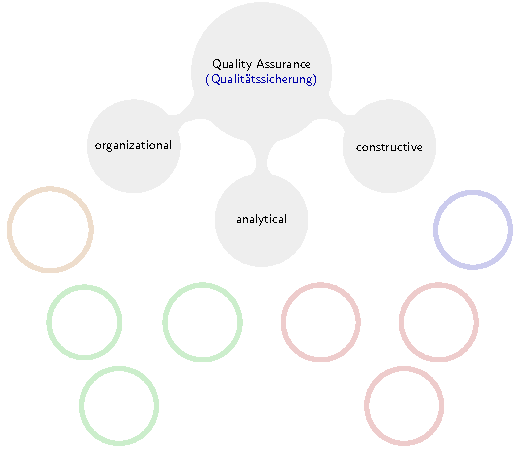
\includegraphics[height=\textheightwithtitle,page=1]{quality-assurance}}%
	\only<2|handout:0>{\includegraphics[height=\textheightwithtitle,page=2]{quality-assurance}}%
	\only<3|handout:0>{\includegraphics[height=\textheightwithtitle,page=3]{quality-assurance}}%
	\only<4|handout:0>{\includegraphics[height=\textheightwithtitle,page=4]{quality-assurance}}%
	\only<5|handout:1>{\includegraphics[height=\textheightwithtitle,page=5]{quality-assurance}}%
	\only<6|handout:0>{\includegraphics[height=\textheightwithtitle,page=6]{quality-assurance}}%
\end{frame}

\begin{frame}{}
	\todo{motivating example that software quality matters, static analysis matters}
\end{frame}

\subsection{Automated Analysis of Product Lines}

\begin{frame}{\myframetitle}
	% properties one might want to analyze, similar to questions about feature models in modeling.tex
	% include questions for all four quadrants
	\todots
	% \begin{mycolumns}
	% 	\mynote{Open Questions}{
	% 		\begin{itemize}
	% 			\item How do such configurators work?
	% 			\item How to avoid inconsistencies?
	% 			\item How to provide explanations and fixes?
    % 			\item How to get all valid configurations automatically? (\emph{P2(b)})
	% 		\end{itemize}
	% 	}
	% 	\mydefinition{Automated Analysis of Feature Models}{
	% 		\begin{itemize}
	% 			\item up until now: \emph{creation} and \emph{transformation} of feature models
	% 			\item now: \emph{analysis} of feature models to improve our understanding of a configuration space
	% 			\item for brevity: product = valid configuration
	% 		\end{itemize}
	% 	}
	% \mynextcolumn
	% 	\myexample{Asking Questions About Product Lines}{
	% 		(in ascending order of difficulty)
	% 		\begin{itemize}
	% 			\item Can we test 
	% 			\item Can we compile every product successfully?
	% 			\item Can we test every product successfully?
	% 			\item 
	% 			\item Is a given configuration valid?
	% 			\item Is there any product at all?\\
	% 				How many/which products are there?\\
	% 			\item Is a given feature (de-)selectable at all?\\
	% 				How many/which products include it?\\
	% 			\item Is a given partial configuration consistent?\\
	% 				How many/which products include it?\\
	% 			\item \color{gray}{(Which features always occur together?)}
	% 			\item \color{gray}{(Is a given constraint redundant?)}
	% 			\item \color{gray}{(How do two feature model versions differ?)}
	% 			\item \color{gray}{(Why is \ldots? How to fix \ldots?)}
	% 		\end{itemize}
	% 	}
	% \end{mycolumns}
\end{frame}

\subsection{Product-Based Analysis Strategies} % refs missing in whole part!

\begin{frame}{\myframetitle}
	\begin{mycolumns}
		\mydefinition{Intuition}{
			\begin{itemize}
				\item to analyze the product line, just analyze \emph{each product}
				\begin{itemize}
					\item individually
					\item in isolation
					\item possibly in parallel
				\end{itemize}
				\item e.g., compile and test each product
			\end{itemize}
		}
		\myexampletight{}{\centering\featureDiagramLego}
	\mynextcolumn
		\pic[width=\linewidth,page=9]{lego-analyses}
	\end{mycolumns}
\end{frame}

\begin{frame}{\myframetitle}
	\begin{mycolumns}
		\mydefinition{Generic Algorithm}{
			\begin{algorithmic}
				\Require a product line $pl$; algorithms $\gamma_p$, $\alpha$, $\sigma$
				\State $C \gets AllSAT(\phi(FM_{pl}))$ \Comment{{\small enumerate valid config's}}
				\State $results \gets []$
				\ForAll{$S \in C$} \Comment{{\small for each valid config}}
				\State $p \gets \gamma_p(S)$ \Comment{{\small generate product}}
				\State $results \pluseq \alpha(p)$ \Comment{{\small add analysis result}}
				\EndFor
				\State \Return $\sigma(results)$
			\end{algorithmic}
		}
		\mynote{}{
			\begin{itemize}
				\item $\gamma_p$ \emph{generates} (e.g., compiles) products (e.g., \texttt{make}, \texttt{gradle}, \texttt{FeatureHouse}, \texttt{npm}, \ldots)
				\item $\alpha$ \emph{analyzes} the product (e.g., run tests)
				\item $\sigma$ \emph{summarizes} the results (e.g., each individual call to $\alpha$ must succeed)
			\end{itemize}
		}
	\mynextcolumn
		\myexampletight{}{
			\begin{center}
				\small\featureDiagramConfigurableDatabase
			\end{center}
		}
		\myexample{}{
			\footnotesize
			\leftandright{
				$\sigma([\alpha(\gamma_p(\{C,G,W\}))$\\
				$~~~~\alpha(\gamma_p(\{C,P,W\}))$\\
				$~~~~\alpha(\gamma_p(\{C,G,P,W\}))$\\
				$~~~~\alpha(\gamma_p(\{C,D,W\}))$\\
				$~~~~\alpha(\gamma_p(\{C,G,D,W\}))$\\
				$~~~~\alpha(\gamma_p(\{C,P,D,W\}))$\\
				$~~~~\alpha(\gamma_p(\{C,G,P,D,W\}))$\\
				$~~~~\alpha(\gamma_p(\{C,P,T,W\}))$\\
				$~~~~\alpha(\gamma_p(\{C,G,P,T,W\}))$\\
				$~~~~\alpha(\gamma_p(\{C,D,T,W\}))$\\
				$~~~~\alpha(\gamma_p(\{C,G,D,T,W\}))$\\
				$~~~~\alpha(\gamma_p(\{C,P,D,T,W\}))$\\
				$~~~~\alpha(\gamma_p(\{C,G,P,D,T,W\}))$
			}{
				$\alpha(\gamma_p(\{C,G,L\}))$\\
				$\alpha(\gamma_p(\{C,P,L\}))$\\
				$\alpha(\gamma_p(\{C,G,P,L\}))$\\
				$\alpha(\gamma_p(\{C,D,L\}))$\\
				$\alpha(\gamma_p(\{C,G,D,L\}))$\\
				$\alpha(\gamma_p(\{C,P,D,L\}))$\\
				$\alpha(\gamma_p(\{C,G,P,D,L\}))$\\
				$\alpha(\gamma_p(\{C,P,T,L\}))$\\
				$\alpha(\gamma_p(\{C,G,P,T,L\}))$\\
				$\alpha(\gamma_p(\{C,D,T,L\}))$\\
				$\alpha(\gamma_p(\{C,G,D,T,L\}))$\\
				$\alpha(\gamma_p(\{C,P,D,T,L\}))$\\
				$\alpha(\gamma_p(\{C,G,P,D,T,L\}))])$
			}
		}
	\end{mycolumns}
\end{frame}

\begin{frame}{Classification of Product-Line Analysis Strategies}
	\begin{mycolumns}[t,columns=3]
		\summaryproductbased
	\mynextcolumn
	\mynextcolumn
	\end{mycolumns}
\end{frame}

\subsection{Feature-Based Analysis Strategies}

\begin{frame}{\myframetitle}
	\begin{mycolumns}
		\mydefinition{Intuition}{
			\begin{itemize}
				\item to analyze the product line, just analyze \emph{each feature} individually
				\item ignore all relations to other features
				\item e.g., test each plug-in, feature module, \ldots
			\end{itemize}
		}
		\myexampletight{}{\centering\featureDiagramLego}
	\mynextcolumn
		\pic[width=\linewidth,page=6]{lego-analyses}
	\end{mycolumns}
\end{frame}

\begin{frame}{\myframetitle}
	\begin{mycolumns}
		\mydefinition{Generic Algorithm}{
			\begin{algorithmic}
				\Require a product line $pl$; algorithms $\gamma_f$, $\alpha$, $\sigma$
				\State $results \gets []$
				\ForAll{$f \in F_{pl}$} \Comment{{\small for each feature}}
				\State $stub \gets \gamma_f(f)$ \Comment{{\small generate feature stub}}
				\State $results \pluseq \alpha(stub)$ \Comment{{\small add analysis result}}
				\EndFor
				\State \Return $\sigma(results)$
			\end{algorithmic}
		}
		\mynote{}{
			\begin{itemize}
				\item $\gamma_f$ \emph{generates} feature stubs (e.g., remove all references to other features)
				\item $\alpha$ \emph{analyzes} the feature stub\\(see product-based)
				\item $\sigma$ \emph{summarizes} the results (see product-based)
			\end{itemize}
		}
	\mynextcolumn
		\myexampletight{}{
			\begin{center}
				\small\featureDiagramConfigurableDatabase
			\end{center}
		}
		\myexample{}{
			\vspace*{-4ex}
			\small
			\begin{align*}
				\sigma([&\alpha(\gamma_f(C)) \text{ -- e.g., compile and test base code}\\
				&\alpha(\gamma_f(G)) \text{ -- e.g., compile and test Get feature}\\
				&\alpha(\gamma_f(P)) \text{ -- \ldots}\\
				&\alpha(\gamma_f(D))\\
				&\alpha(\gamma_f(T))\\
				&\alpha(\gamma_f(W))\\
				&\alpha(\gamma_f(L))])
			\end{align*}
		}
	\end{mycolumns}
\end{frame}

\begin{frame}{Classification of Product-Line Analysis Strategies}
	\begin{mycolumns}[t,columns=3]
		\summaryproductbased
	\mynextcolumn
		\summaryfeaturebased
	\mynextcolumn
	\end{mycolumns}
\end{frame}

\subsection{Family-Based Analysis Strategies}

\begin{frame}{\myframetitle}
	\begin{mycolumns}
		\mydefinition{Intuition}{
			\begin{itemize}
				\item to analyze the product line, generate and analyze a single \emph{metaproduct}
				\item the metaproduct encodes all variability in one large product, which can then be analyzed
				\item the metaproduct then contains the feature model, all feature mappings, \ldots
			\end{itemize}
		}
		\myexampletight{}{\centering\featureDiagramLego}
	\mynextcolumn
		\pic[width=\linewidth,page=3]{lego-analyses}
	\end{mycolumns}
\end{frame}

\begin{frame}{\myframetitle}
	\begin{mycolumns}
		\mydefinition{Generic Algorithm}{
			\begin{algorithmic}
				\Require a product line $pl$; algorithms $\gamma_{mp}$, $\alpha$
				\State $p \gets \gamma_{mp}(FM_{pl}, F_{pl})$ \Comment{{\small generate metaproduct}}
				\State \Return $\alpha(p)$ \Comment{{\small analyze metaproduct}}
			\end{algorithmic}
		}
		\mynote{}{
			\begin{itemize}
				\item $\gamma_{mp}$ \emph{generates} the metaproduct (e.g., encode \texttt{\#ifdef}'s as runtime variability)
				\item $\alpha$ \emph{analyzes} the metaproduct\\(see product-based)
			\end{itemize}
		}
	\mynextcolumn
		\myexampletight{}{
			\begin{center}
				\small\featureDiagramConfigurableDatabase
			\end{center}
		}
		\myexample{}{
			\vspace*{-4ex}
			\small
			\begin{align*}
				\alpha(\gamma_{mp}(\ldots)) &\text{ -- e.g., compile and test everything at once}\\
				&\text{ (how can this be done?)}
			\end{align*}
		}
	\end{mycolumns}
\end{frame}

\subsection{Classification of Analysis Strategies}

\begin{frame}{\myframetitle}
	\begin{mycolumns}[t,columns=3]
		\summaryproductbased
	\mynextcolumn
		\summaryfeaturebased
	\mynextcolumn
		\summaryfamilybased
	\end{mycolumns}
\end{frame}